\chapter{Evaluation of the ICE--Model}\label{modelanalysis}
We now have a complete geomtrical representation of the ICE model as well as
 the analytical expressions $u_0$ and $u_L$ that describe the membrane displacements
in spatial detail as a function of direction and frequency. In this chapter we will use these variables
to further study the features of our model and compare them with experimental results.

We start in Sec \ref{vibrationpatternchapter} by comparing the experimentally determined vibration pattern
of the Tokay gecko's eardrum with that of our model's eardrum. In Sec. \ref{pressuredistchapter} we will
briefly discuss the pressure distribution profile and eigenfrequencies of our cavity.
In Sec \ref{hearingcueschapter} we will define and study the two main quantities that serve as important localization
cues - the Internal Time Differene (iTD) and the Internal Level Difference (iLD). These values model the
neural subtraction taking place in the animal's brain which is the final step in localization. This
is in contrast to the Interaural Time and Level Differences (ITD and ILD) that are
entirely determined by the inputs to the two ears.


\subsubsection{Parameter Estimation}
Before we begin our analysis, we need to give numerical values to the parameters we first defined
in \ref{parametertable}. To do this we will simultaneously need to use experimentally determined
values and estimate physical quantities that haven't been measured based on experimental results. 
In our study we are primarily concerned with hearing in geckos. We will be using
parameters (interaural separation, tympanum area etc.) from \textit{Hemidactylus frenatus}, the common house gecko
\cite{dalsgaardmanley2}
and the Tokay gecko \cite{dalsgaardmanley1}, \cite{dalsgaardtangcarr}. The paramters are listed for both these
species in Table \ref{geckogeometricparams}.

\begin{minipage}{\linewidth}
\renewcommand{\arraystretch}{1.2}
%\caption{Parameters and Functions used in the ICE Model} \label{parametertable} 
\centering
\captionof{table}{Geometry Parameters for the common house gecko (Hemidactylus frenatus) estimated from \cite{dalsgaardmanley2}
and the Tokay gecko obtained from \cite{dalsgaardmanley1} and \cite{dalsgaardtangcarr}.} \label{geckogeometricparams} 
\begin{tabular}{|p{8.5 cm} | c | c|}
\hline
Parameter name & Hemidactylus & Tokay gecko\\
\hline
Length of the cylinder or interaural distance, L & $10$mm & $22$mm\\
Radius of the tympanic membrane, $a_{tymp}$& $1.2$mm & $2.2$mm\\
Fundamental frequency (first eigenfrequency) of the tympanic membrane, $\omega_{01}$ & $2800$Hz & $1700$Hz\\
Quality factor of the tympanum, $Q$ & $1.2$ &  $1.2$\\
Density of the membrane material, $\rho_m$ & $1$mg/mm$^3$ & $1$mg/mm$^3$\\
Thickness of the membrane, $d$& $8\mu$m & $10\mu$m\\
Volume of the cavity, $V_0$ & $.32$ml & $3.5$ml\\ 
Extracolumella angle, $\beta$ & $\pi/25$ & $\pi/25$\\
\hline
\end {tabular}\par
\bigskip
\end{minipage}

As we can see, the house gecko, with an interaural separation of $10$mm and mouth cavity volume of $.32$ml is a rather
small lizard. The Tokay gecko is the second largest gecko species (interaural separation of $25.6$mm and mouth cavity volume $3.5$ml, \cite{dalsgaardtangcarr}).
Thus we will demonstrate the applicability of our model to animals hearing with widely varying head widths and mouth cavities. The geometric parameters, especially
the head width and the membrane eigenfrequencies put important limits on the ``hearing range'' of our model as we will see in Sec. \ref{hearingcueschapter}.

\section{Spatial Vibration Pattern of the Membrane}\label{vibrationpatternchapter}
We begin our analysis by evaluating the variation of the spatial vibration pattern of the tympanic membrane
with frequency. The tympanic vibration pattern was first measured experimentally by Manley \cite{manleygecko1}
for a \textit{Tokay gecko} and was found to have the strongest response at around 1kHz. The measured vibration patterns
are shown on the left in Fig. \ref{manleygeckotympanum}. Manley measured the vibration amplitude for eight locations on the membrane and measured the pattern
seen on the left of Fig. \ref{manleygeckotympanum}. As we can see, at around $4$kHz, the vibration pattern
distinctly develops two maxima - something that would not happen to a centrally loaded tympanum except
at frequencies well beyond the hearing range of geckos.

\begin{figure}[ht!]
 \centering
 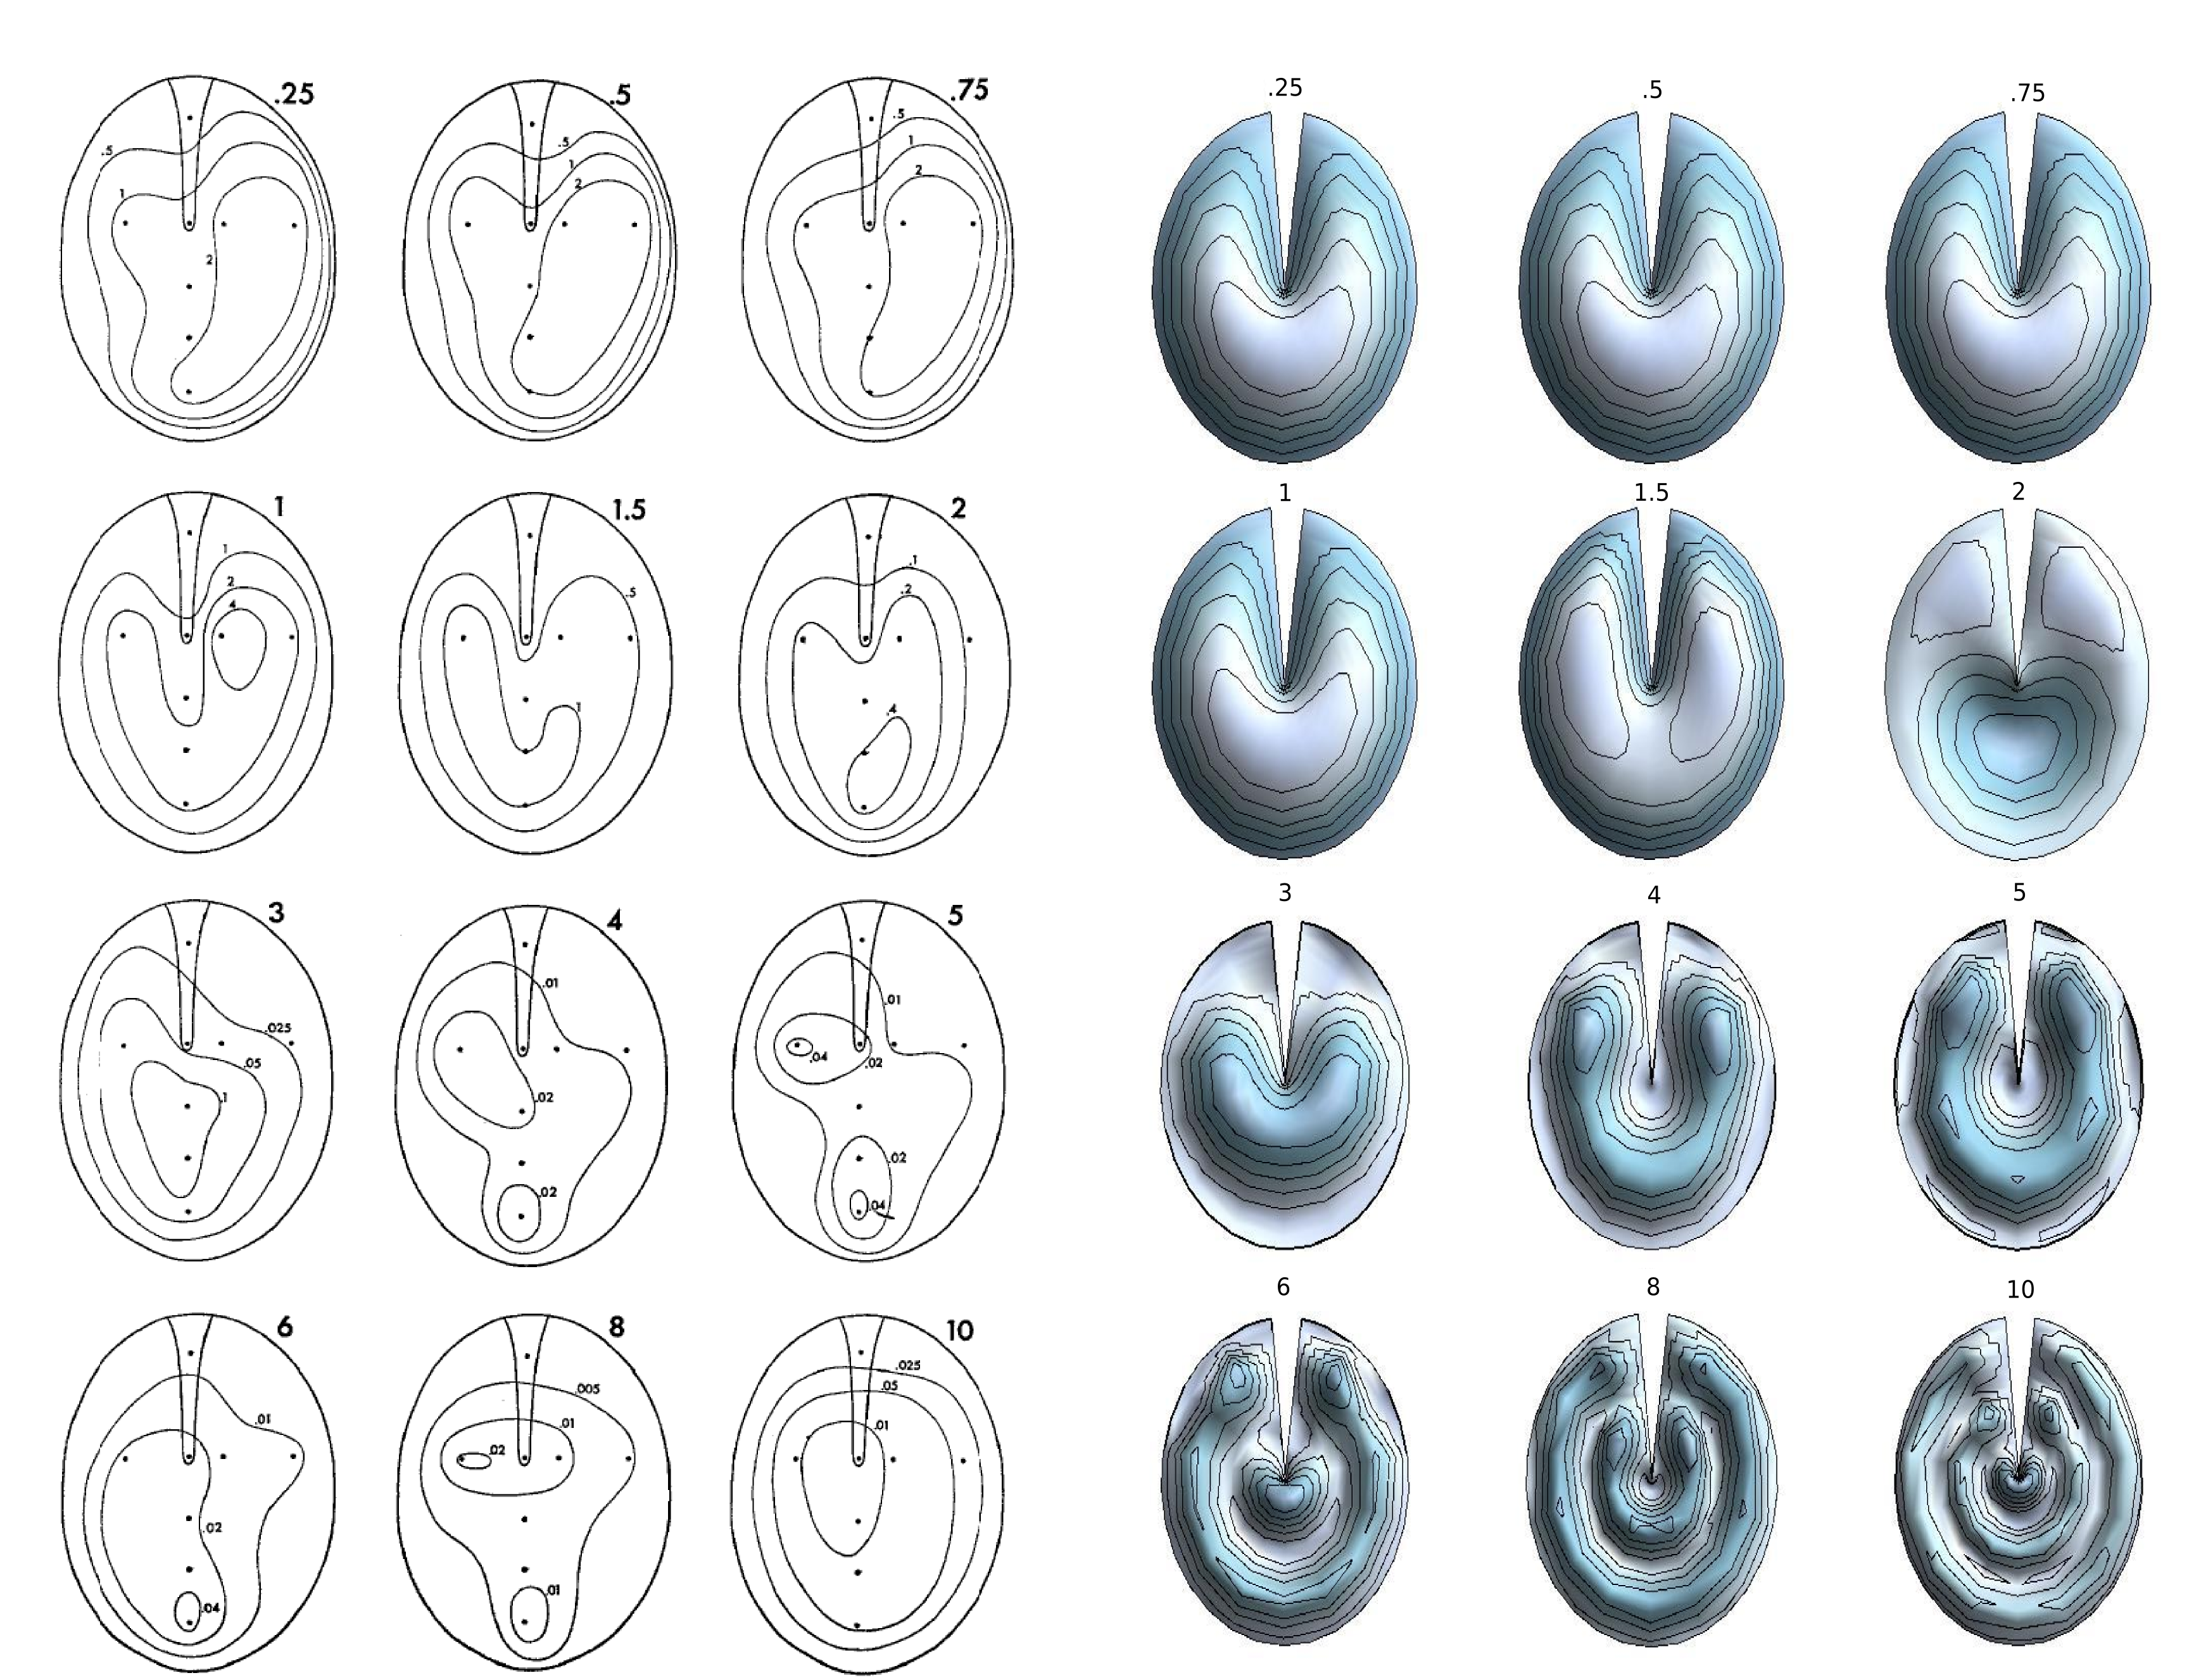
\includegraphics[width=1.0\linewidth]{Diagrams/manleymodelcomparison.png}
 \caption[Tokay gecko tympanum vibration profiles.]{Experimental membrane vibration patterns of the Tokay gecko dependent
 on sound frequency varying from $.5$kHz to $10$kHz. Data taken from \cite{manleygecko1}.}
  \label{manleygeckotympanum}
\end{figure}

In order to compare our model with the experimental results, we plot the response of the ipsilateral membrane in our cylindrical ICE model 
calculated using \eqref{ipsimembranefull}. The input was chosen to be purely ipsilateral, meaning $p_L=0$. 
This is illustrated in Fig. \ref{manleygeckotympanum} (right) for the same frequency range as in the experimental data. The ipsilateral input was chosen to have unit amplitude and the model parameters used are given
on the right most column of Table \ref{geckogeometricparams}. The omitted region corresponds to the extracolumella. 

The asymmetric nature of our membrane vibration pattern is a result of our chosen geometry.
Mathematically this is a result of the fact that a uniform pressure (on the membrane surface) on a full circular membrane only couples to the circularly symmetric $J_0$ modes.
In the case of the sectoral membrane however, the uniform pressure couples to all the eigenmodes resulting in a more complex pattern.
As a qualitative reproduction our model is very accurate but for a full quantitative analysis, we would 
need to account for the motion of the extracolumella. Moreover, the full mechanics of the extracolumella would 
also include its flection at higher frequencies.
% \begin{figure}[ht!]
%  \centering
%  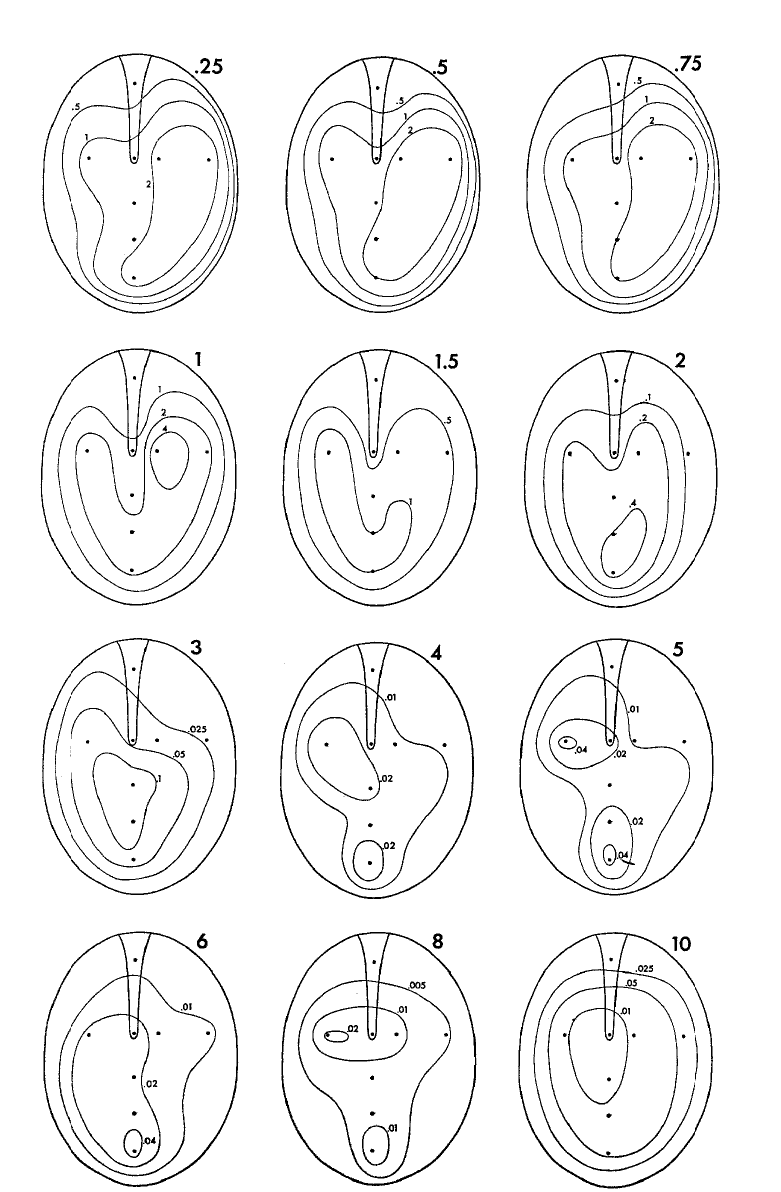
\includegraphics[width=.5\linewidth]{Diagrams/manleygeckoear2.png}
%  \caption[Tokay gecko tympanum vibration profiles.]{Experimental membrane vibration patterns of the Tokay gecko dependent
%  on sound frequency varying from $.5$kHz to $10$kHz. Data taken from \cite{manleygecko1}.}
%   \label{manleygeckotympanum}
% \end{figure}

% \begin{figure}[ht!]
%  \centering
%  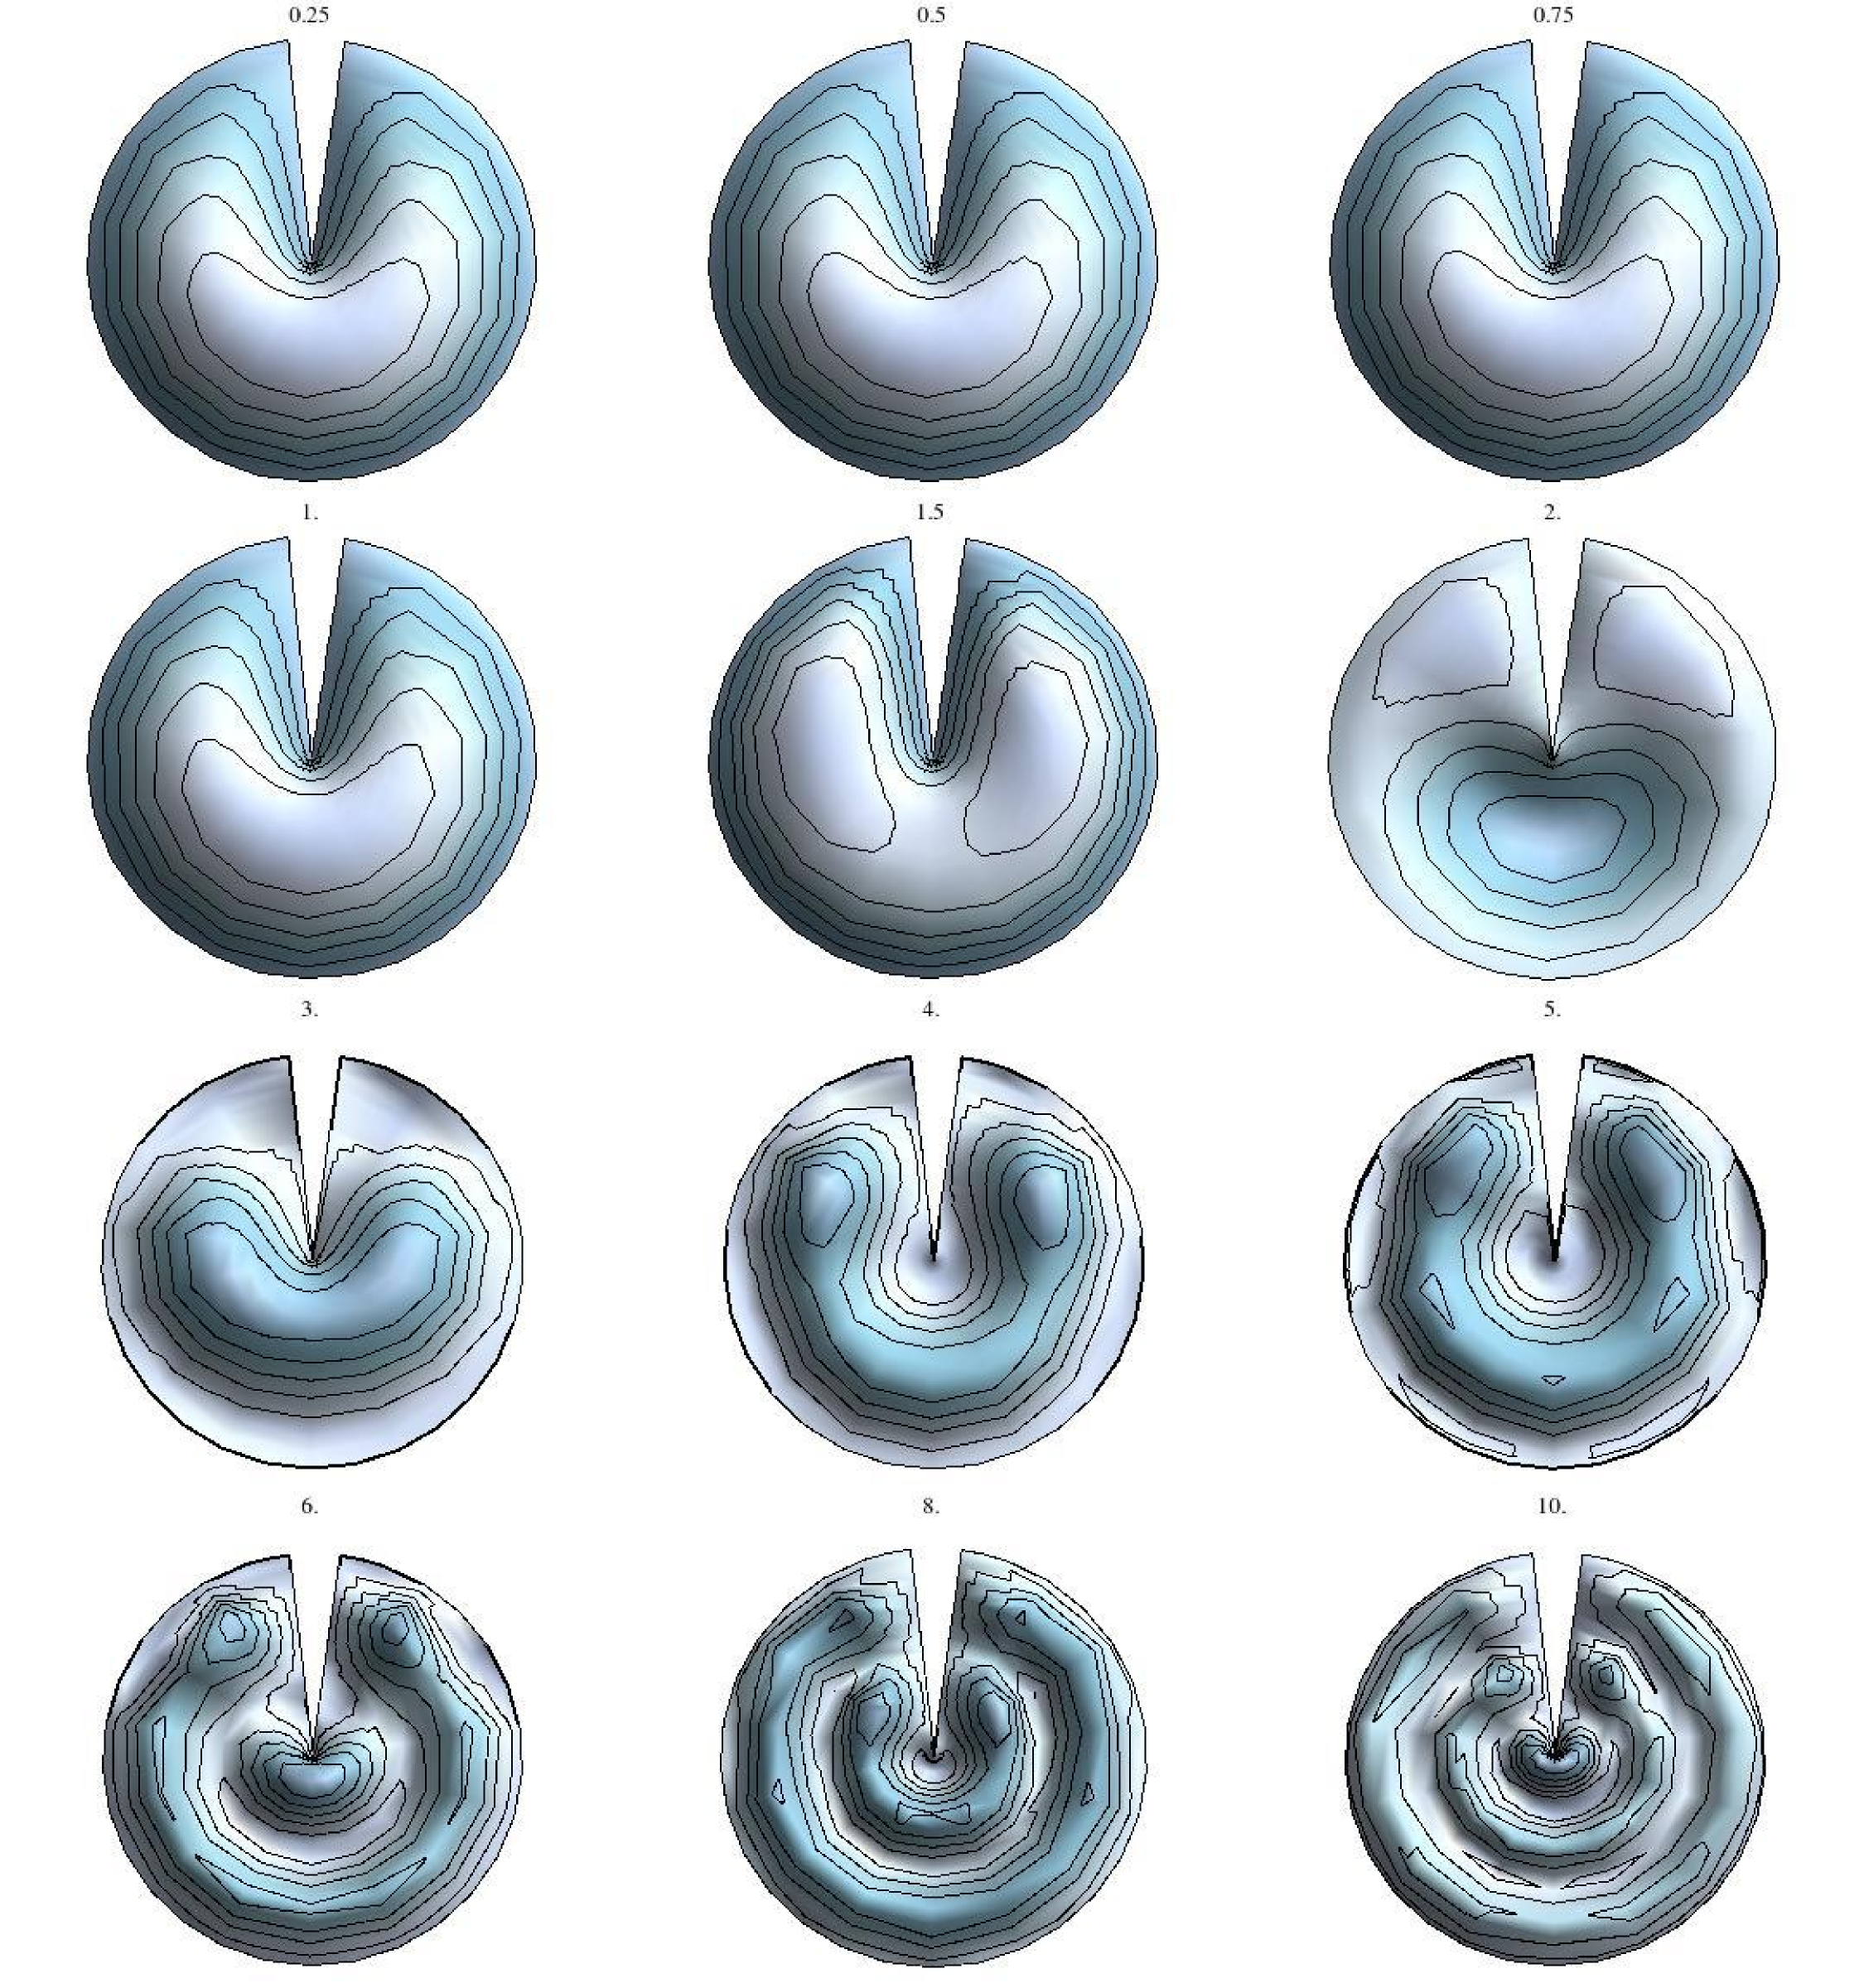
\includegraphics[width=.75\linewidth]{Diagrams/SectorMembraneModes/sector_membrane_all.png}
%  \caption[Sectoral membrane vibration profiles.]{Vibration patterns of a sectoral membrane
%  of radius $2.2$mm on sound frequency varying from $.5$kHz to $10$kHz. Compare with fig. \ref{manleygeckotympanum}}
%   \label{sectormembraneprofile}
% \end{figure}

\section{Cavity Pressure Distribution}\label{pressuredistchapter}

\section{Directional Hearing Cues}\label{hearingcueschapter}

\subsection{Transmission Gain}

\subsection{Internal Time Difference}

\subsection{Internal Level Difference}